\begin{figure}[h]
\centering
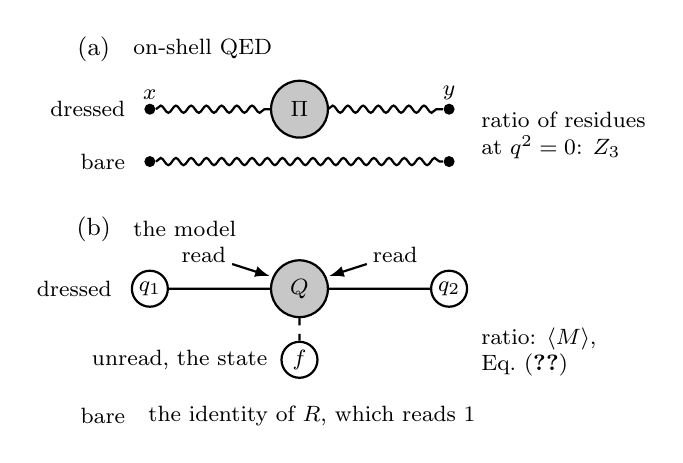
\begin{tikzpicture}[scale=0.95, every node/.style={font=\footnotesize},
  photon/.style={decorate, decoration={snake, amplitude=1.3pt, segment length=5.5pt}, thick},
  ins/.style={circle, fill=black, inner sep=0pt, minimum size=4pt},
  qd/.style={circle, draw, thick, fill=white, inner sep=0pt, minimum size=13pt}]
% (a) on-shell QED
\node[font=\small] at (-0.75,1.15) {(a)};
\node[anchor=west] at (-0.35,1.15) {on-shell QED};
\node[anchor=east] at (-0.2,0.35) {dressed};
\node[ins] (x) at (0,0.35) {}; \node[ins] (y) at (4,0.35) {};
\draw[photon] (x) -- (1.62,0.35);
\draw[photon] (2.38,0.35) -- (y);
\draw[thick, fill=black!22] (2,0.35) circle (0.38);
\node at (2,0.35) {$\Pi$};
\node[above] at (x) {$x$}; \node[above] at (y) {$y$};
\node[anchor=east] at (-0.2,-0.35) {bare};
\node[ins] (xb) at (0,-0.35) {}; \node[ins] (yb) at (4,-0.35) {};
\draw[photon] (xb) -- (yb);
\node[anchor=west, align=left] at (4.3,0) {ratio of residues\\at $q^{2}=0$: $Z_{3}$};
% (b) the model
\node[font=\small] at (-0.75,-1.25) {(b)};
\node[anchor=west] at (-0.35,-1.25) {the model};
\node[anchor=east] at (-0.38,-2.05) {dressed};
\node[qd] (q1) at (0,-2.05) {$q_{1}$};
\node[qd] (q2) at (4,-2.05) {$q_{2}$};
\draw[thick, fill=black!22] (2,-2.05) circle (0.38);
\node at (2,-2.05) {$Q$};
\draw[thick] (q1) -- (1.62,-2.05);
\draw[thick] (2.38,-2.05) -- (q2);
\draw[-latex, thick] (1.1,-1.72) -- (1.6,-1.88); \node at (0.72,-1.6) {read};
\draw[-latex, thick] (2.9,-1.72) -- (2.4,-1.88); \node at (3.28,-1.6) {read};
\node[qd] (f) at (2,-3.0) {$f$};
\draw[thick, dashed] (2,-2.43) -- (f);
\node[anchor=east] at (1.7,-3.0) {unread, the state};
\node[anchor=west, align=left] at (4.3,-2.9) {ratio: $\langle M\rangle$,\\Eq.~(\ref{eq:alpha})};
\node[anchor=east] at (-0.2,-3.75) {bare};
\node[anchor=west] at (-0.15,-3.75) {the identity of $R$, which reads $1$};
\end{tikzpicture}
\caption{A correspondence of roles, not of diagrams. (a)~In on-shell QED, $Z_{3}$ is the residue at $q^{2}=0$ of the dressed photon two-point function, two field insertions at $x$ and $y$ joined through every vacuum-polarization insertion (shaded), over that of the bare one. (b)~The model's counterpart in the object of Fig.~\ref{fig:link}(a), with the two read links drawn apart: the two reads, taken at the shared qutrit $Q$ on the links to $q_{1}$ and $q_{2}$, are the two insertions, the unread link to $f$ carries the state, the bare insertion is the identity of $R$, and the dressed insertion $M$ weighs the $172$ records at $Q$ (shaded), Eq.~(\ref{eq:alpha}) of the Letter. No record is a Feynman diagram. The model has no charged loop, no vertex factor, no loop momentum, and no expansion in a coupling, and the identification of the object with the photon is the Photon Conjecture.}
\label{fig:s-roles}
\end{figure}
